\section{Technologie abordées}
  \begin{frame}
    \frametitle{Technologies abordées}
    \begin{itemize}
      \item Jxta : réseau Pair-à-Pair
      \item Dart
      \item HTML5 + Javascript
      \item GWT
    \end{itemize}
  \end{frame}

  \subsection*{Jxta : réseau Pair-à-Pair}
    \begin{frame}
      \frametitle{Jxta : réseau Pair-à-Pair}
      \begin{itemize}
        \item Technologie open source.
        \item Permettant de faire un réseau	pair-à-pair en Java. 
        \item Le  réseau pair-à-pair est créé sur le réseau existant permettant aux différents noeuds de pouvoir communiquer entre eux.\\
      \end{itemize}
    \end{frame}
    
    \begin{frame}
      \frametitle{Jxta : réseau Pair-à-Pair}
      	\begin{figure}
			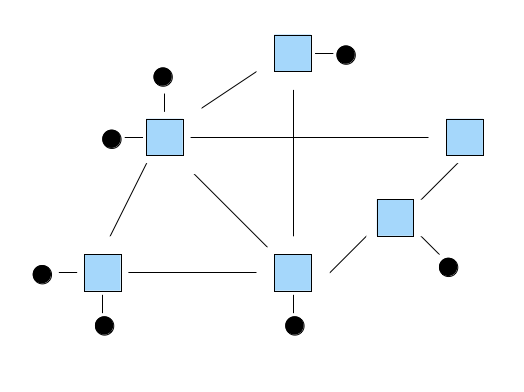
\includegraphics[scale=0.3]{includes/network-model.png}
	   	\end{figure}
    \end{frame}

  \subsection*{Dart}
    \begin{frame}
      \frametitle{Dart}
      \begin{itemize}
        \item Pouet
      \end{itemize}
    \end{frame}

  \subsection*{HTML5 + Javascript}
    \begin{frame}
      \frametitle{HTML5 + Javascript}
      \begin{itemize}
        \item Pouet
      \end{itemize}
    \end{frame}

  \subsection*{GWT}
    \begin{frame}
      \frametitle{GWT}
      \begin{figure}
		\center
		
\includegraphics[scale=0.60]{gwt-logo}
	  \end{figure}
      \begin{itemize}
        \item Google Web Toolkit
        \item Framework développé par Google
        \item<2->Compatible multi navigateur
        \item<3-> Java vers Javascript
        \item<4->Fonction native 
      \end{itemize}
    \end{frame}

